% !TEX root = Dokumentation_SysSpec.tex
\subsection{Externe Schnittstellen}
\subsubsection{Rollen und Akteure}
Im Rahmen des Filial-Bestellsystems existieren folgende Akteure, welche zugleich spezifische Rollen und somit Berechtigungen besitzen.
\begin{itemize}
	\item Benutzer: Jeder Akteur in der Rolle 'Benutzer' kann sich am System mit den entsprechenden Zugangsdaten anmelden.
	\item Filialleiter: besitzt die Rechte 'OrderView' und 'OrderEdit' und kann daher sowohl bestehende Bestellungen einsehen, bearbeiten und annullieren.
	\item Verkaufspersonal: hat grundsätzlich identische Rechte wie Filialleiter, kann jedoch zusätzlich noch Bestellungen erfassen. TODO: Prüfen, ob wirklich so umgesetzt!
	\item Datentypist: besitzt die Rolle 'Supply' und kann dadurch den Wareneingang im System erfassen
	\item Filialverwalter: besitzt die Rolle 'LogView' und kann daher das Logfile mit den abgelaufenen Systemabläufen überprüfen. Die Einsicht via Filial-Bestellsystem in das Logfile ist nicht im Release 1.0 realisiert. In folgenden Releases wird über eine zentrale Logfile-Verwaltung (bspw. Syslog) entschieden. 
	\item Sysadmin: hat keine aktiven Steuerungsmöglichkeiten innerhalb des Systems. Der Anwendungsfall des Sysadmins ist für Release 1.0 noch nicht definiert.
\end{itemize}
\subsubsection{Datenbankanbindung}
TODO Tobias: OR-Mapper Anbindung beschreiben\\

Für die Persistierung der Daten (ausser Logdaten, RW und Zentrallager) wird eine MySQL-Datenbank aus dem EnterpriseLab mit dem folgenden ConnectionString verwendet:
- TODO ConnectionString
Auf Stufe Datenbank wurden keine weiteren Sichten, Prozeduren und Benutzer eingesetzt. Daher wird gegenüber der Datenbank nur der User grp13 verwendet.
\subsubsection{Zentrallager}
Für das Zentrallager wird eine Stock-Schnittstelle zur Verfügung gestellt. Sie ist in einem Maven-Repo ('https://bintray.com/hslu/maven/appe/5.0.1\#files/ch/hslu/appe/appe\_stock') abgelegt und bereits in das Modul 'appe\_layer\_business' integriert.\\
Die detaillierte Dokumentation zur vorgegebenen Schnittstelle ist unter\\
'https://elearning.hslu.ch/ilias/ilias.php?ref\_id=3290529\&page=APPE\_Startseite\&wpg\_id=11071\&cmd=downloadFile\&cmdClass=ilwikipagegui\&cmdNode=yi:l5:yk\&baseClass=ilwikihandlergui\&file\_id=il\_\_file\_3582976' zu beziehen.

Die Implementation wurde im Business-Layer vorgenommen. Die vorgegebene Schnittstelle wurde nur in einem minimalen Ausmass verwendet. Im Rahmen einer Bestelländerung /-erfassung wird bei Unterschreiten der definierten Mindestanzahl eines Artikels (bis Release 1.0 fix auf 2 definiert) über die Methode 'orderArticle(....)' eine Nachbestellung in der Höhe der geforderten Artikel + 2 ausgelöst. Es wird dabei nicht geprüft, ob am Zentrallager noch entsprechende Artikel vorhanden sind. \\Es wird daher davon ausgegangen, dass am Zentrallager wie auch im Filiallager ein Negativlagerbestand möglich ist. Die Schnittstelle ist dadurch nur unidirektional und es werden keine Daten \& Interaktionen durch das Zentrallager an das Filial-Bestellsystem direkt ausgeführt.  \\
TODO Severin: Klassendiagram hinzufügen
\subsubsection{Rechnungswesen}
Das Rechnungswesen hat die Aufgabe bei Erfassung / Änderung einer Bestellung eine entsprechende Rechnung an den Kunden zu versenden.\\
Von Seiten Auftraggeber sind keine Schnittstellen zur Verfügung gestellt worden und daher wurden die entsprechenden Aufgaben des Rechnungswesen als simpler Stub implementiert, der lediglich ein Output über die ausgeführte Arbeit (z.B. Neue Rechnung gedruckt) protokolliert. \\
TODO Severin: Klassendiagram hinzufügen

\subsection{Interne Schnittstellen}
In diesem Kapitel werden nur wichtige, systemrelevante Schnittstellen spezifiziert. Es werden primär die Schnittstellen zwischen den Layern 'Client', 'Business' inkl. Remote und 'Data' beschrieben.

\subsubsection{Globale Sicht}
In einer groben Übersicht wird die globale Sicht der Schnittstellen zwischen den Schichten / Packages aufgezeigt.:\\
\begin{figure}[H]
\centering
	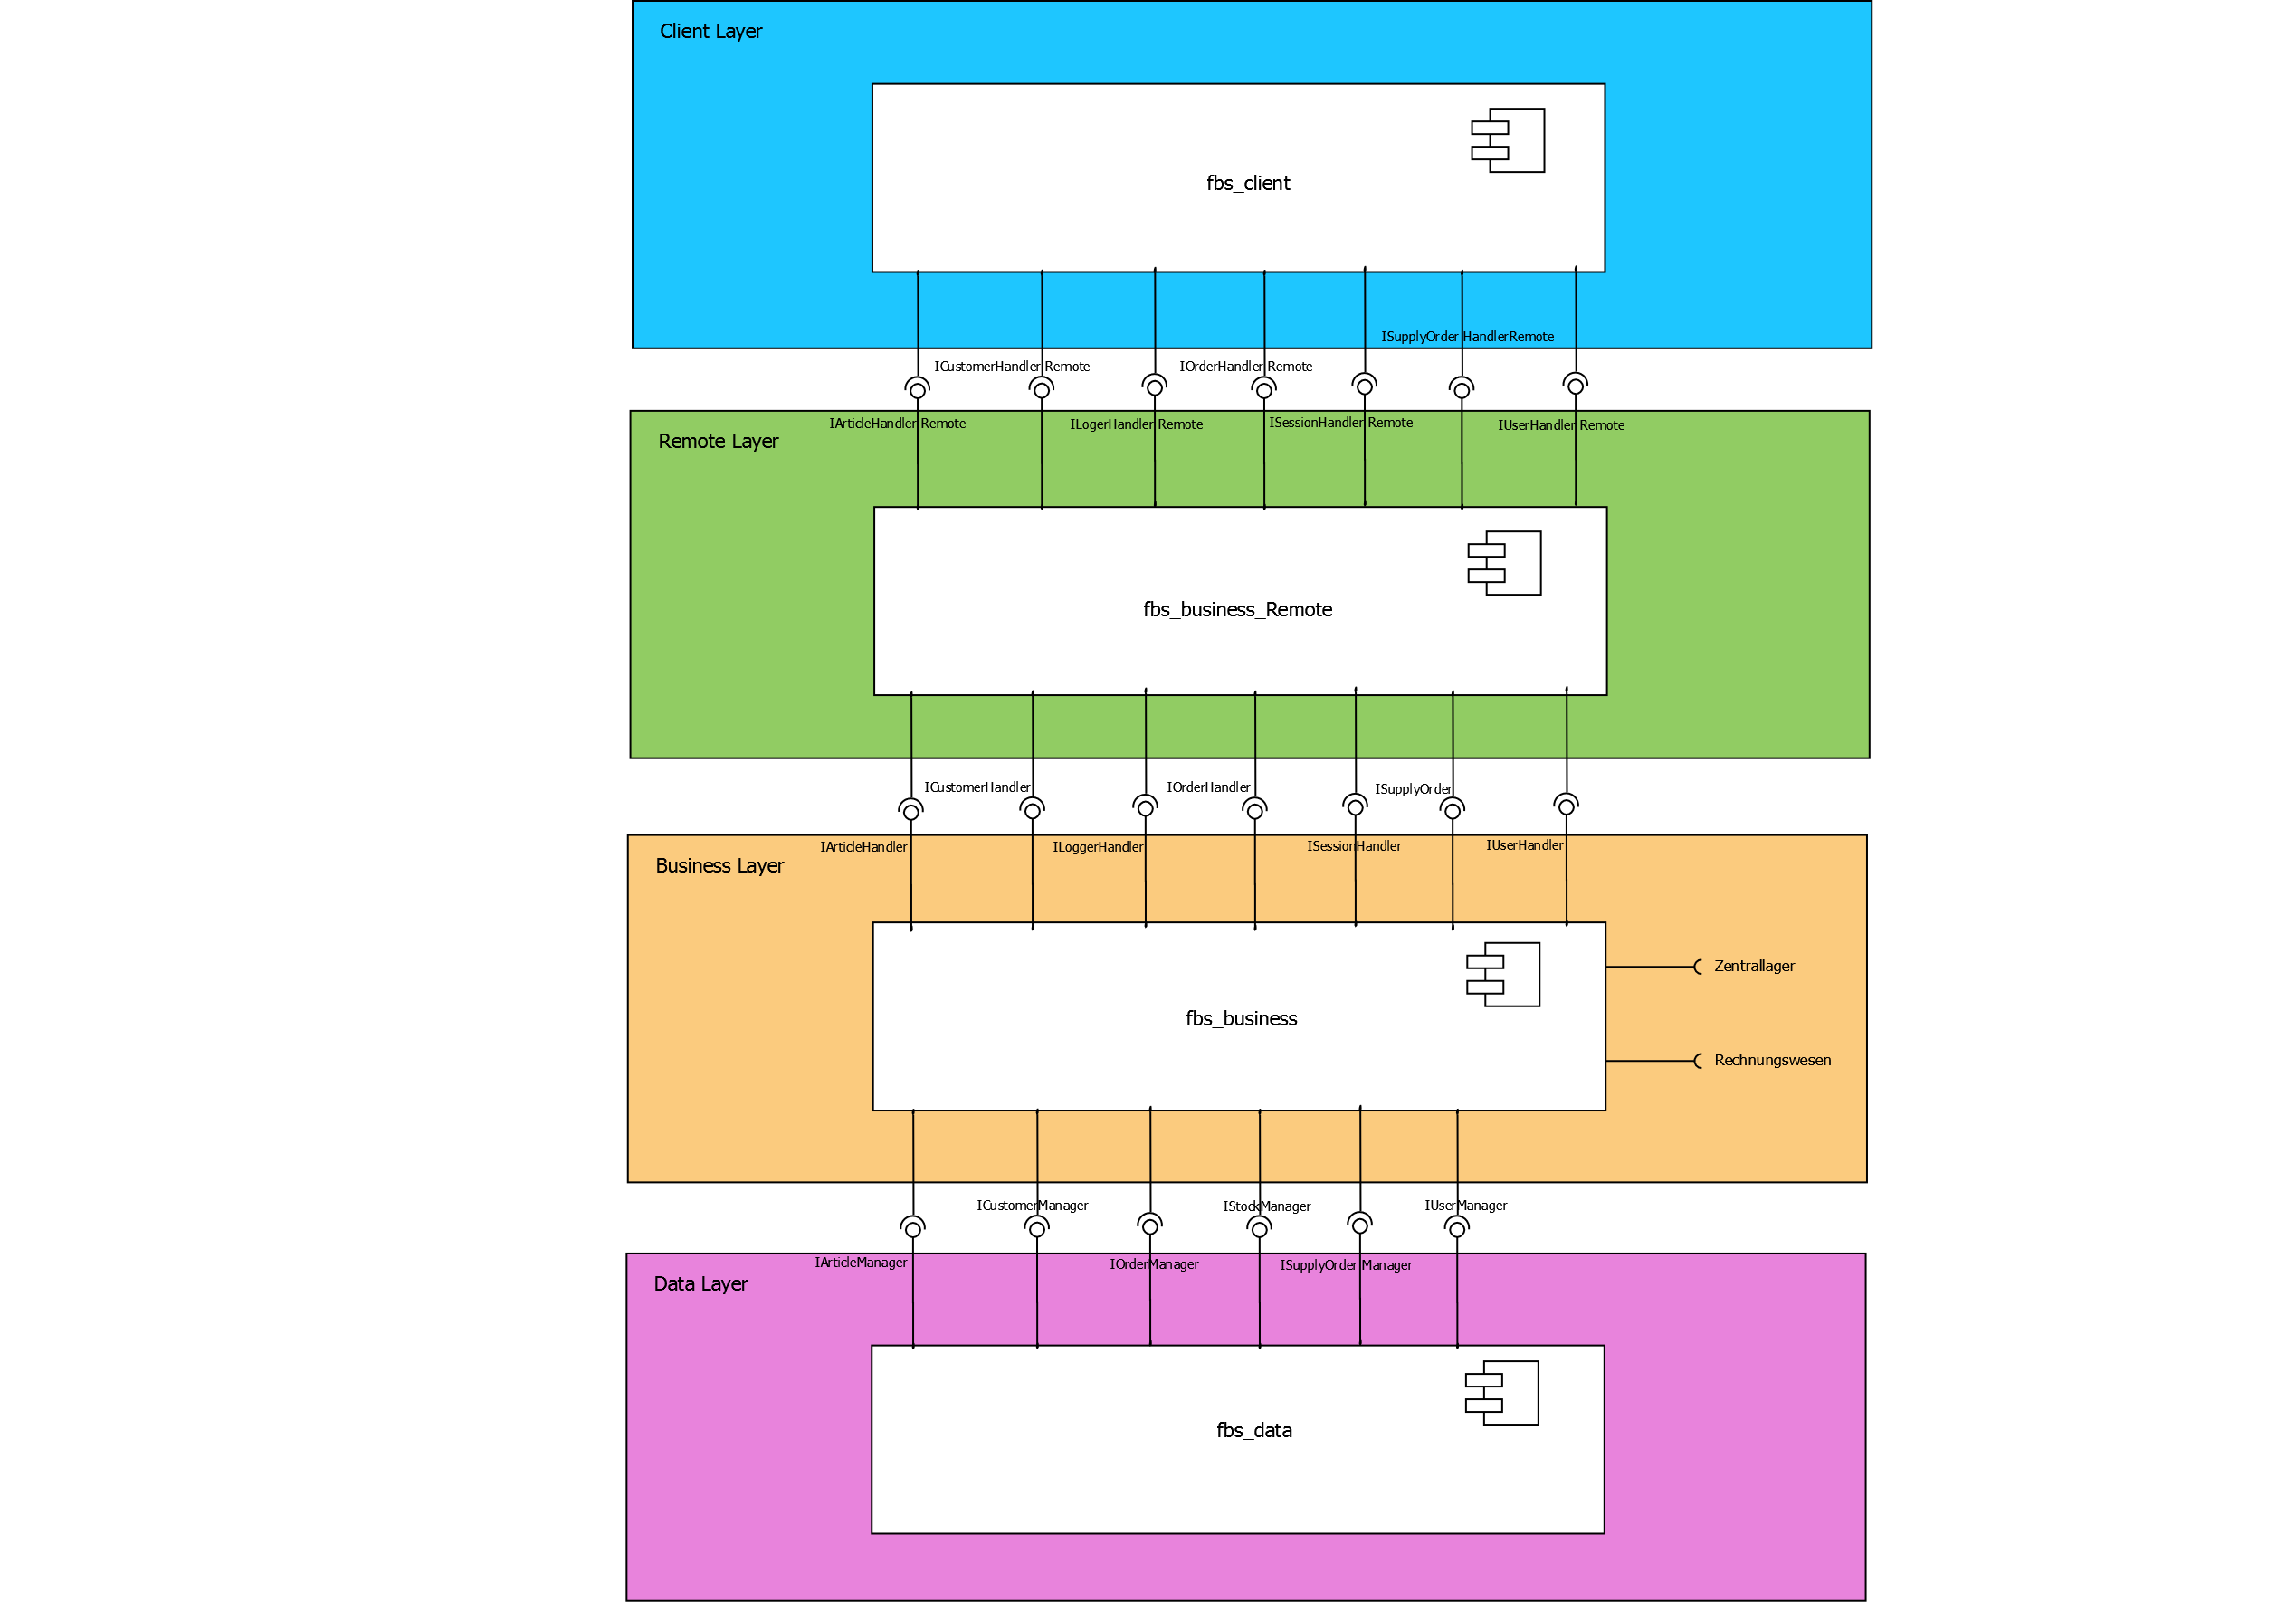
\includegraphics[width=1.0\linewidth]{Images/Schnittstellen}
	\caption{Schnittstellen}
	\label{fig:schnittstellen}
\end{figure}

\subsubsection{Client <-> Remote}
Der Client-Layer ist generell als MVC implementiert. Der Controller fordert bei Aktionen des Benutzers jeweils die nachgefragten Informationen über die Remote-Schicht an, und sendet neue und geänderte Bestellungen über die definierten Schnittstellen zur Remote-Schicht.
Der Client-Layer strukturiert die erhaltenen Daten in einem eigenen Model transient ab.
TODO Klassendiagramme hinzufügen, eventuell Sequenz-Diagram

Speziell ist das User- und Session-Management. Der User erhält auf Basis der über die Login-Schnittstelle erhaltenen Benutzergruppe seine Berechigung zugewiesen. Diese Zuweisung wird im Singelton-Pattern des Users abgespeichert.
Das Singleton-Pattern wird dabei benötigt, um den Kontext des Benutzers auf Business-Ebene zu prüfen.
TODO Klassendiagram hinzufügen

Die Kontext-Prüfung wird dabei über eine dedizierte Schnittstelle zu Beginn jedes Aufrufes eingeleitet. So werden ungültige Aufrufe verhindert.
TODO Klassendiagramme Hnzufügen

Der Login-Prozess der Applikation entscheidet auf Basis der erhaltenen Benutzergruppe, welche Ansicht der jeweilige Benutzer erhält. Diese Entscheidung ist dabei über ein Strategy-Pattern implementiert. 
TODO Klassendiagramme Hnzufügen

Die Implementation des Client-Layers beruht auf JavaFX, bzw. FXML. Diese Implementation erzwingt den Einsatz von Observable-Objekten.

Der Client ist stark von der Remote-Schicht der Business-Logik abhängig. Es ist nicht gedacht, dass der Client-Layer für andere Applikationen verwendet wird.
\newline

------------------------------------------------------------------
\textbf{IOrderHandlerRemonte}\\
Über die Methode 'getOrder' unter Angabe der gewünschten Bestellnr (int) wird vom Business Layer die Bestellung als 'OrderDTO' bereitgestellt. Für die Auflistung aller Bestellungen wird die Methode 'getOrderList' verwendet.\\
Unter Angabe der Bestellnummer kann eine Bestellung annulliert werden (Methode cancelOrder(int)). Für das Ändern oder Speichern einer Bestellung werden zusätzlich Informationen (z.B. Kunden, bestellte Artikel) benötigt, weshalb ein OrderDTO benötigt wird.


\begin{figure}[H]
	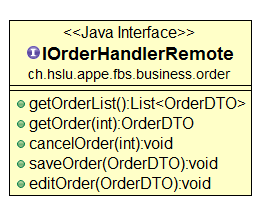
\includegraphics[width=0.3\linewidth]{Images/IOrderHandlerRemonte}
	\caption{Interface IOrderHandlerRemonte}
	\label{fig:if-IOrderHandlerRemonte}
\end{figure}

\textbf{ISupplyOrderHandlerRemonte}\\
Für die Auflistung aller Nachbestellungen wird die Methode 'getFullOrderList' verwendet und liefert ein SupplyOrderDTO zurück.\\
Mittels der Methode 'updateSupplyFromArrical' wird mit der Übergabe eines 'SupplyOrderDTO' eine Nachbestellung ausgelöst. 
\begin{figure}[H]
	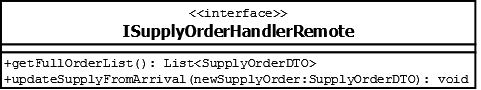
\includegraphics[width=0.6\linewidth]{Images/ISupplyOrderHandlerRemonte}
	\caption{Interface ISupplyOrderHandlerRemonte}
	\label{fig:if-ISupplyOrderHandler}
\end{figure}


\textbf{IArticleHandlerRemonte}\\
Für die Auflistung aller möglicher Artikel wird die Methode 'getFullArticleList' verwendet und liefert alle Liste aller verfügbaren Artikel zurück. Alle Artikel einer spezifischen Bestellung kann über 'getOrderArticleList' abgefragt werden. Sie benötigt eine ordernr (int). Ein einzelner Artikel kann über 'getArticle' mit Übergabe einer articleNr von der Remonteschicht angefordert werden. Die genannte Anzahl sind nicht garantiert, sondern zeigt lediglich einen Momentanbestand. Das Transaktionsmanagement unterliegt den unteren Layers.
\begin{figure}[H]
	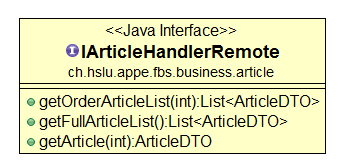
\includegraphics[width=0.6\linewidth]{Images/IArticleHandlerRemonte}
	\caption{Interface IArticlerHandlerRemonte}
	\label{fig:if-IArticleHandlerRemonte}
\end{figure}

\textbf{ICustomerHandlerRemonte}\\
Beim ICustomerHandlerRemonte wird bis Release 1.0 keine erstellende oder mutierende Operationen angeboten. Konkret heisst dies, dass über 'getCustomerList' alle möglichen Kunden ausgewiesen werden und über eine Liste 'CustomerDTO' zurückgegeben. Es besteht mittels customerNr auch die Möglichkeit einen selektiven Kunden zu erhalten. Dies geschieht mit der Methode 'getCustomer'.
Die Methode 'getCustomerStateOK' überprüft, ob der Kunden ausstehende Mahnungen hat und liefert einen boolean (true=OK / false=Mahnung) zurück.
\begin{figure}[H]
	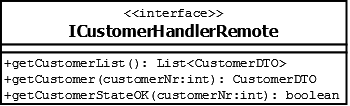
\includegraphics[width=0.4\linewidth]{Images/ICustomerHandlerRemonte}
	\caption{Interface ICustomerHandlerRemonte}
	\label{fig:if-ICustomerHandler}
\end{figure}

\textbf{IUserHandlerRemonte}\\
Über das IUserHandlerRemonte-Interface kann Abgefragt werden ob ein User gültig ist und das richtige Passwort eingegeben wurde. Mit 'getUserRole' kann anhand des Username seine Rolle abgefragt werden, z.B. für die Auswahl der Ziel-Page. 
\begin{figure}[H]
	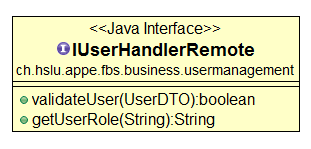
\includegraphics[width=0.4\linewidth]{Images/IUserHandlerRemonte}
	\caption{Interface IUserHandlerRemonte}
	\label{fig:if-IUserHandlerRemonte}
\end{figure}


\textbf{ISessionHandlerRemonte}\\
Die Schnittstelle 'ISessionHandlerRemonte' überprüft, ob der User die Berechtigungen für den gewünschten Ziel-Context hat oder nicht. Bei jedem Pageaufruf, wird die Überprüfung für jede Page (LoginPage ausgenommen) vorgenommen.
\begin{figure}[H]
	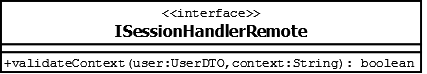
\includegraphics[width=0.5\linewidth]{Images/ISessionHandlerRemonte}
	\caption{Interface ISessionHandlerRemonte}
	\label{fig:if-ISessionHandlerRemonte}
\end{figure}

\textbf{ILoggerHandlerRemonte}\\
Das ILoggerHandlerRemonte-Interface bietet die möglichkeit anhand eines LogerDTO eine LogMessage zu übergeben. Die LogLevels werden in der unteren Schicht bestimmt. Es wird ein Default wert festgelegt für alle Lognachrichten vom Clint Layer.
\begin{figure}[H]
	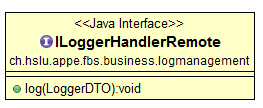
\includegraphics[width=0.5\linewidth]{Images/ILoggerHandlerRemonte}
	\caption{Interface ILoggerHandlerRemonte}
	\label{fig:if-ILoggerHandler}
\end{figure}


\subsubsection{Remote <-> Business}
Zwischen der Anbindung der Layer 'Remote' und 'Business' existieren ähnliche Schnittstellen wie bei 'Client <-> Remote'. Diese Schicht reicht die Client-Operationsanfragen mit notwendiger Datentransformation (DTO zu Model) an den entsprechenden Business-Handler.\\\\
\textbf{IOrderHandler}\\
Über die Methode 'getOrder' unter Angabe der gewünschten Bestellnr wird vom Data-Layer die Bestellung als 'OrderModel' bereitgestellt. Für die Auflistung aller Bestellungen wird die Methode 'getOrderList' verwendet.\\
Unter Angabe der Bestellnummer kann eine Bestellung annulliert werden (Methode cancelOrder). Für das Ändern oder Speichern einer Bestellung werden zusätzlich Informationen (z.B. Kunden, bestellte Artikel) benötigt, weshalb ein OrderModel benötigt wird. 
\begin{figure}[H]
	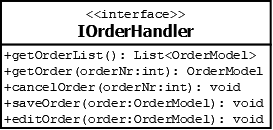
\includegraphics[width=0.3\linewidth]{Images/IOrderHandler}
	\caption{Interface IOrderHandler}
	\label{fig:if-IOrderHandler}
\end{figure}
\textbf{ISupplyOrderHandler}\\
Für die Auflistung aller Nachbestellungen wird die Methode 'getFullOrderList' verwendet.\\
Mittels der Methode 'changeLocalArticleStockAmount' wird überprüft, ob der Filiallagerbestand für jeden einzelnen Artikel unter den Mindestbestand fällt und löst bei Unterschreitung eine Bestellung beim Zentrallager aus. Die Methode 'setCurrentSupplyOrder' ermöglicht anhand der auslösenden Bestellung eine provisorische Nachbestellung zu erstellen. Alle nachzubestellende Artikel werden dieser Nachbestellung beigefügt. Nachdem alle Nachbestellartikel erfasst sind, muss diese über 'saveSupply' an den Data-Layer für die Persistierung gesendet werden. Die Methode 'updateSupplyFromArrival' wird beim Wareneingang verwendet, um angelieferte Artikel zu verbuchen. 
\begin{figure}[H]
	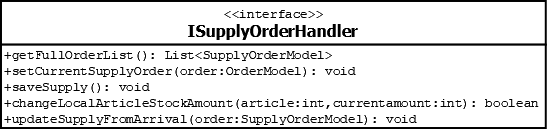
\includegraphics[width=0.6\linewidth]{Images/ISupplyOrderHandler}
	\caption{Interface ISupplyOrderHandler}
	\label{fig:if-ISupplyOrderHandler}
\end{figure}
\clearpage
\textbf{IArticleHandler}\\
Für die Auflistung aller möglicher Artikel (z.B. im NewOrder-Form) wird die Methode 'getFullArticleList' verwendet. Ein einzelner Artikel kann über 'getArticle' unter Artikelnummer von der Datenbank angefordert werden. Über 'getArticleAmountFromStock' kann pro Artikel der aktuelle Filiallagerbestand abgefragt werden. Die genannte Anzahl ist nicht garantiert, sondern zeigt lediglich einen Momentanbestand. Neben dem Auslesen der Artikelmenge wird über die Methode 'updateArticleAmount' die Möglichkeit zur Aktualisierung der Artikelmenge angeboten. Das Transaktionsmanagement unterliegt ausschliesslich dem Data-Layer, da über die Methode nur die gewünschte Mengendifferenz übertragen wird.
\begin{figure}[H]
	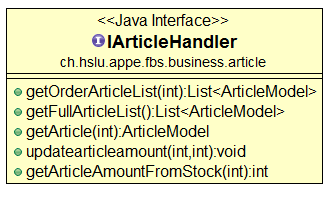
\includegraphics[width=0.6\linewidth]{Images/IArticleHandler}
	\caption{Interface IArticlerHandler}
	\label{fig:if-IArticleHandler}
\end{figure}

\textbf{ICustomerHandler}\\
Beim ICustomerHandler wird bis Release 1.0 keine erstellende oder mutierende Operationen angeboten. Konkret heisst dies, dass über 'getCustomerList' alle möglichen Kunden ausgewiesen werden. Es besteht mittels Kundennummer auch die Möglichkeit einen selektiven Kunden zu erhalten (Methode 'getCustomer).\\
Die Methode 'getCustomerStateOK' überprüft beim FinanceStub, ob der Kunden ausstehende Mahnungen hat und so nicht legitimiert ist Bestellungen zu tätigen.
\begin{figure}[H]
	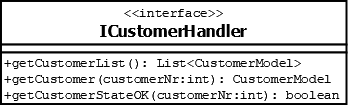
\includegraphics[width=0.4\linewidth]{Images/ICustomerHandler}
	\caption{Interface ICustomerHandler}
	\label{fig:if-ICustomerHandler}
\end{figure}
\textbf{IUserHandler}\\
Über das IUserHandler-Interface können die Userinformationen (Benutzername, Passwort und Userrolle) erfragt werden. Die Userrolle kann ebenfalls für einen bestimmten Benutzer separat erfragt werden, z.B. für die Auswahl der Ziel-Page im Client.
\begin{figure}[H]
	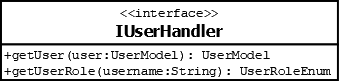
\includegraphics[width=0.4\linewidth]{Images/IUserHandler}
	\caption{Interface IUserHandler}
	\label{fig:if-IUserHandler}
\end{figure}
\clearpage
\textbf{ISessionHandler}\\
Die Schnittstelle 'ISessionHandler' überprüft, ob der User die Berechtigungen für den gewünschten Ziel-Context hat oder nicht. Bei jedem Pageaufruf, wird die Überprüfung für jede Page (LoginPage ausgenommen) vorgenommen.
\begin{figure}[H]
	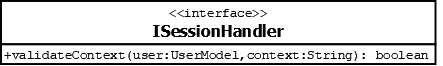
\includegraphics[width=0.5\linewidth]{Images/ISessionHandler}
	\caption{Interface ISessionHandler}
	\label{fig:if-ISessionHandler}
\end{figure}
\textbf{ILoggerHandler}\\
Das ILoggerHandler-Interface bietet anhand eines LoggerModels, welches bereits die Nachricht und Level enthält, zu übermitteln oder kann mittels dem Enum LogLevelEnum den Level und die Message als String vorgeben.
\begin{figure}[H]
	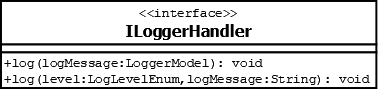
\includegraphics[width=0.5\linewidth]{Images/ILoggerHandler}
	\caption{Interface ILoggerHandler}
	\label{fig:if-ILoggerHandler}
\end{figure}



\subsubsection{Business <-> Data}
TODO Marco \&Tobias
